% !TEX root = root.tex
\chapter{\label{chap:trackpy}Software Development: A Modern Particle-Tracking Toolkit}
\chaptermark{Software}

A large portion of my thesis effort has been devoted to the development of particle tracking and data analysis software, dubbed ``trackpy,'' used for my own soft matter research and the work of others in our group. It is also being adopted by other soft matter researchers at Harvard, Princeton, Oxford, U. Chicago, U. Penn, and more. Relying on the growing open-source scientific software community, I have leveraged free, widely-used code for core functionality. By contributing my own particle tracking and data analysis code back to the community, I have increased the impact of the work and encouraged others to share their own improvements to my code, from which all users benefit.

Trackpy integrates with a fast-growing tool from this community: a standardized, browser-based notebook of multilingual code with figures, explanatory text and equations, and links and references. As recently highlighted in \emph{Nature}\cite{Shen2014}, these notebooks are making data analysis easier to record, understand, and reproduce. A growing number of authors are publishing these notebooks alongside papers, providing the detail that is essential for others to reproduce the work in a reasonable time scale.

Several researchers have merged their independent efforts into this code. I personally am responsible for implementing feature-finding, motion analysis tools (various statistics and plots), uncertainty estimation, streaming capability (i.e., processing unlimited data sets), and the bulk of the tests and documentation. Thomas A. Caswell wrote the original trajectory-linking code, and Nathan C. Keim contributed the prediction framework, major performance improvements, and improved trajectory linking.

\section{Introduction}

Particle tracking is an extremely powerful technique used across many disciplines of science. It has matured over the past three decades into a broadly accessible technique. Early applications were in cellular biophysics\cite{Schnapp1988,Ghosh1994} and fundamental colloid science\cite{Crocker1996}. More recently, it has been used to directly image atomic rearrangements in silica glass\cite{Huang2013a}; to image stress and strain in drying colloidal films\cite{Xu2013a}; to image pleats in crystals on curved surfaces\cite{Irvine2010}. This broad variety of applications calls for a flexible toolkit that can be adapted for use with a range of data analysis strategies. Making the methods used in various pockets of the literature usable in a single framework increases the reusability of those methods, makes them easier for researchers to discover, and fights the creeping fragmentation of science.

\section{Review of the Crocker--Grier Particle Tracking Algorithm}

Trackpy implements the tracking algorithm of Crocker and Grier\cite{Crocker1996}. Theirs and similar algorithms\cite{Ghosh1994} have been widely used in the fields of colloid science, microrheology, biophysics, and biometrical engineering. The particle-tracking algorithm implemented by Crocker and Grier is performed in two steps: locating the particles in each frame and identifying the particles through time, linking coordinates into trajectories.

Particle coordinates are identified in four steps: 1) preparing the image using common image-processing techniques; 2) finding local maxima of brightness that may correspond to particles; 3) honing in on each candidate particle's exact center with subpixel precision; and 4) discerning which of the candidates are true particles based on their morphology and measured brightness.

The software first prepares the images by applying a spatial bandpass filter, which uses a Fourier transform of the image to suppress features with small-scale variation (e.g., camera noise) and large-scale variation (e.g., uneven lighting). This effectively erases any objects in the background that are much smaller or much larger than the size of the particles. Next, the software identifies all local maxima in the processed image. These do not necessarily correspond to the particles' centers, but they provide an initial estimate of where particles may be found. If two or more local maxima are separated by a distance smaller than the particle diameter, they are assumed to belong to the same particle, and the software only retains the brightest one. Then, the software finds the intensity-weighted centroid (analogous to a center of mass) of each spot, which is refined through iterative steps, using the whole region of the particle to resolve its center to a precision much better than a pixel. (Subpixel resolution is discussed at length in Section \ref{sec:subpx}.) Finally, the software characterizes the neighborhood surrounding each spot by its total brightness, size, and eccentricity (deviation from circular shape). Using these attributes, blobs that correspond to actual particles can be distinguished --- and the rest discarded --- with minimal user input. For example, true colloidal spheres tend to appear bright and circular.

At this point, the algorithm has identified the locations of particles in each frame. Next, the locations must be linked together across frames into particle trajectories. The algorithm robustly handles the complications of real trajectories: particles may leave the field of view, new particles may enter, and particles can even be tracked if they temporarily vanish and reappear nearby within some specified window of time. If particles are well separated and moving slowly relative to the frame rate, the task of linking them is simple and unambiguous. If there are many particles in the field of view and they are moving quickly, the Crocker--Grier linking algorithm assigns particles in a way that minimizes the total length of the links. This is grounded in the statistics of random walks; a Brownian particle is most likely to be found near where it was last seen. The algorithm is rigorously correct for non-interacting Brownian particles\cite{Crocker1996}, and it is employed effectively in a variety of tracking applications.

As the number of particles in view grows, resolving ambiguous networks is difficult. To simplify the problem, the algorithm requires the user to specify the maximum displacement allowed from one frame to the next. A good choice can simply be obtained by watching the particles and guessing the upper range of their movement between frames. Then, after trajectory linking is complete, the choice can be validated by verifying that the distribution of observed particle displacements decays short of this cutoff value, that it is not clipped.

One the appropriate parameters for feature size, appearance, and maximum displacement have been decided, a standard personal computer can typically process at least one video frame per second, though this depends on the number of particles (and therefore the number of calculations needed for a single frame) in view.

\section{Trackpy: An Enhanced Implementation of Crocker--Grier}

Many others have reimplemented the Crocker--Grier algorithm in various languages. (See table in Appendix A.) Our Python implementation is distinguished by succinct and flexible usage, modular design, scalability to data sets of unlimited size, a thorough testing framework ensuring code stability and accuracy, and thorough documentation.

To summarize some key features:
\begin{itemize}

\item Wherever possible, existing tools from widely-used Python modules are employed. Therefore, core functionality such as common image processing routines are supported and tested by a community of scientists much larger than the particle-tracking community.

\item Alongside trackpy, we developed a utility for reading sequential images called PIMS (Python Image Sequence). PIMS handles video data from many formats with one consistent interface, abstracting away the I/O details. It is designed to process videos of unlimited size, pulling data into memory only as it is needed.

\item Results from trackpy are returned as DataFrames, high-performance spreadsheet-like objects that enable powerful and convenient data grouping and reduction operations for ``medium data,'' analogous to the capabilities of relational database systems such as Structure Query Language (SQL).

\item To verify correctness and project stability, a suite of more than 180 tests reproduces basic results (Section \ref{sec:testing}).

\item Both feature-finding and trajectory-linking can be performed on arbitrarily long videos using a fixed, modest amount of memory. (Results can be read and saved to disk throughout.)

\item A prediction framework helps track particles in fluid flows, or other scenarios where velocity is correlated between time steps (Section \ref{sec:prediction}).

\item Feature-finding and trajectory-linking works on images with any number of dimensions, making possible some creative applications.

\item Uncertainty is estimated following a method described in a detailed study by Savin and Doyle\cite{Savin2005} (Section \ref{sec:subpx}).

\item High-performance components---numba acceleration and FFTW (``Fastest Fourier Transform in the West'')---are used only if available. Since these can be tricky to install on some machines, the code will automatically fall back on slower pure Python implementations.

\item Over fifty pages of collaboratively-written documentation with tutorials and examples is provided in Appendix A. The documentation is also, of course, available online.\cite{trackpy}

\end{itemize}


\section{\label{sec:subpx}Subpixel precision and accuracy}

Understanding the precision and accuracy of particle location is critical for conducting reliable particle tracking experiments. In fact, failure to recognize and account for imprecision and inaccuracy in tracking data can lead to qualitative misinterpretation\cite{Deschout2014,Parthasarathy2012} as random errors in particle position can become large systematic errors in derived quantities.

Tracking resolution is different than microscope resolution. As classically defined, microscope resolution is the minimum distance between two distinguishable points. The resolution of a traditional light microscope is approximately 250 nm, half the wavelength of visible light\cite{Thompson2002}. However, this limit does not apply to locating the center of one isolated point. Using an appropriate algorithm, it is possible to locate the center of an isolated particle or point source to better than the diffraction-limited resolution \cite{Bobroff1986,Deschout2014}. In fact, researchers can routinely track particles with a lateral spatial precision of tens of nanometers or less using a standard light microscope\cite{Crocker2007}.

How is it possible to locate a particle's center to better than pixel resolution? If a particle is only visible as one bright pixel, then we can only say that the particle is located somewhere in that pixel. But, if the particle's image spans multiple pixels---ideally, more than three pixels across---we can find its position with subpixel accuracy by taking the average position of these pixels, weighted by brightness. Figure \ref{fig:true-measured-subpx} shows how this is realized by trackpy, comparing the measured positions to actual positions on simulated images where the ground truth is known. On real data, where the ground truth is not known, subpixel accuracy can be checked by looking at the distribution of the decimal parts of the particle positions---that is, position modulo 1 pixel. If the algorithm is not achieving good sub pixel precision, the distribution will often be distorted, typically biased toward pixel edges. Usually this means that the area being used to compute the centroid is too small \cite{Crocker2007}. As demonstrated in Figure \ref{fig:true-measured-subpx}, enlarging that area can improve precision.

   \begin{figure}
    \centering
    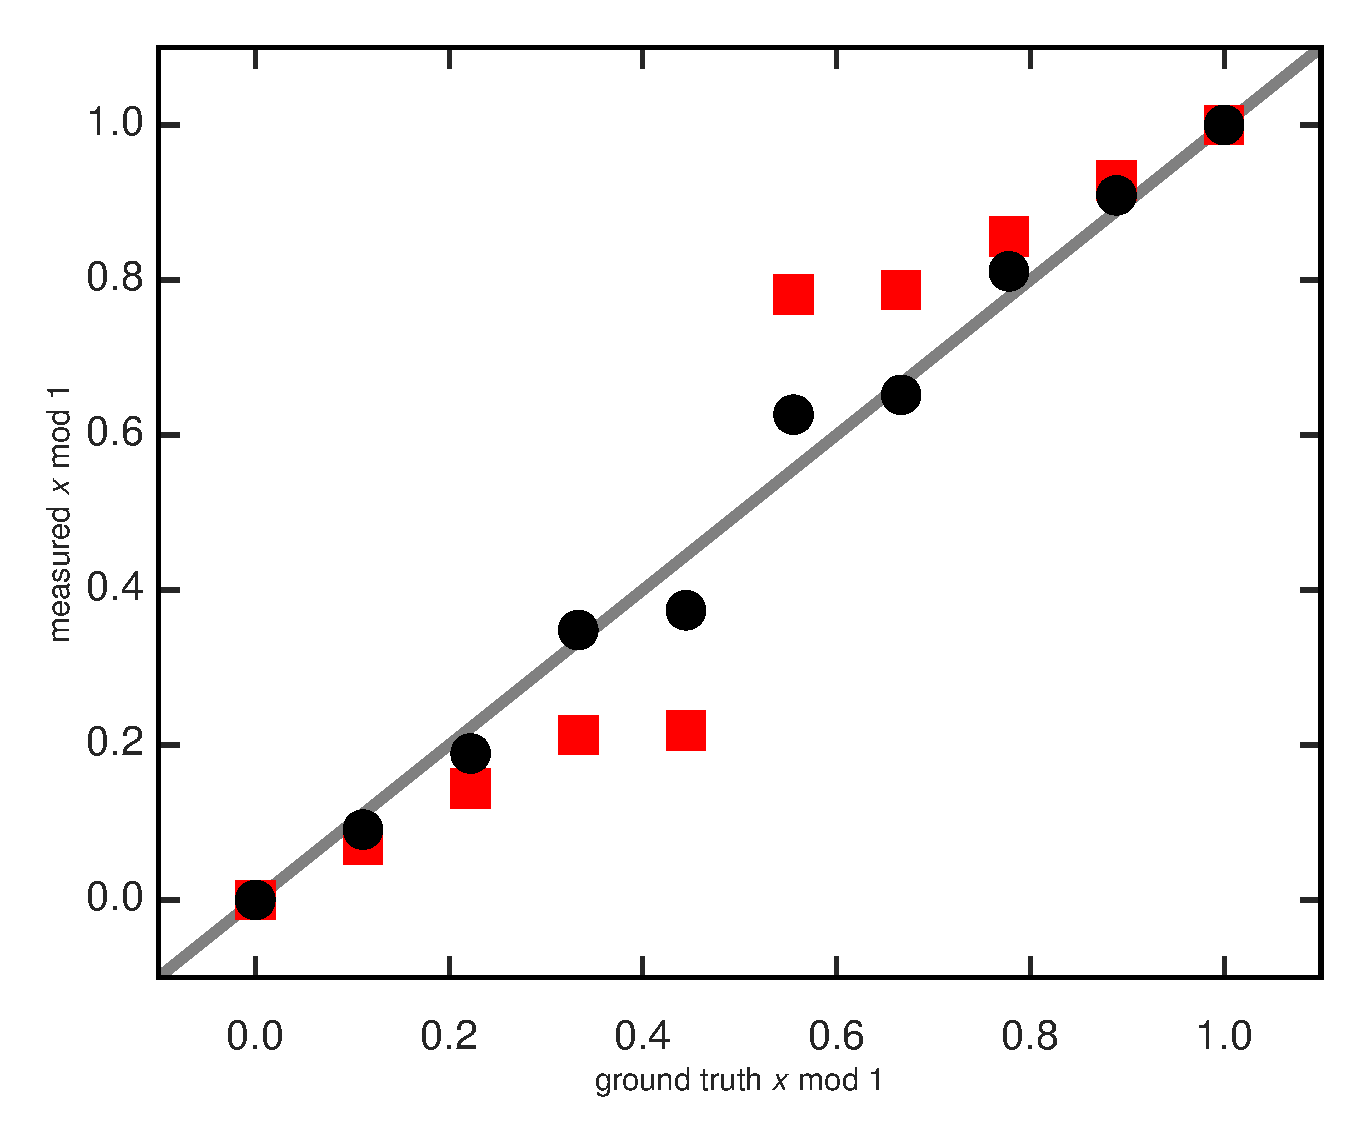
\includegraphics[width=\columnwidth]{trackpy/true-measured-subpx}
    \caption{\label{fig:true-measured-subpx}The decimal part of the $x$ coordinate reveals sub pixel accuracy. Here the measured $x$ coordinate is plotted against the ground truth. When the mask does not cover the edges of the feature, sub pixel accuracy is poor (red squares). In particular, the location is biased toward pixel edges. With a larger mask, accuracy is good to about a tenth of a pixel (black circles).}
    \end{figure}

\subsection{Static Error}

Uncertainty in particle location is variously referred to as static error, localization error, or random error\cite{Savin2005,Martin2002a,Crocker1996}. Tracking precision is subject to both fundamental and experimental limitations. The fundamental limitation is photon noise: a particle emits photons stochastically, and consequently, there is statistical uncertainty in locating the particle from its image. The size of this uncertainty is inversely proportional to the square root of the number of detected photons\cite{Ober2004}. Experimental limitations related to detector and specimen properties can also degrade precision. Detector noise, including dark current (thermally-induced electrons in the detector) and readout noise (errors in reading the number of photoelectrons built up in a pixel), can interfere with particle localization\cite{Thompson2002,Deschout2012}. Image processing can remove some, but not all, of this background\cite{Deschout2014}.

   \begin{figure}
    \centering
    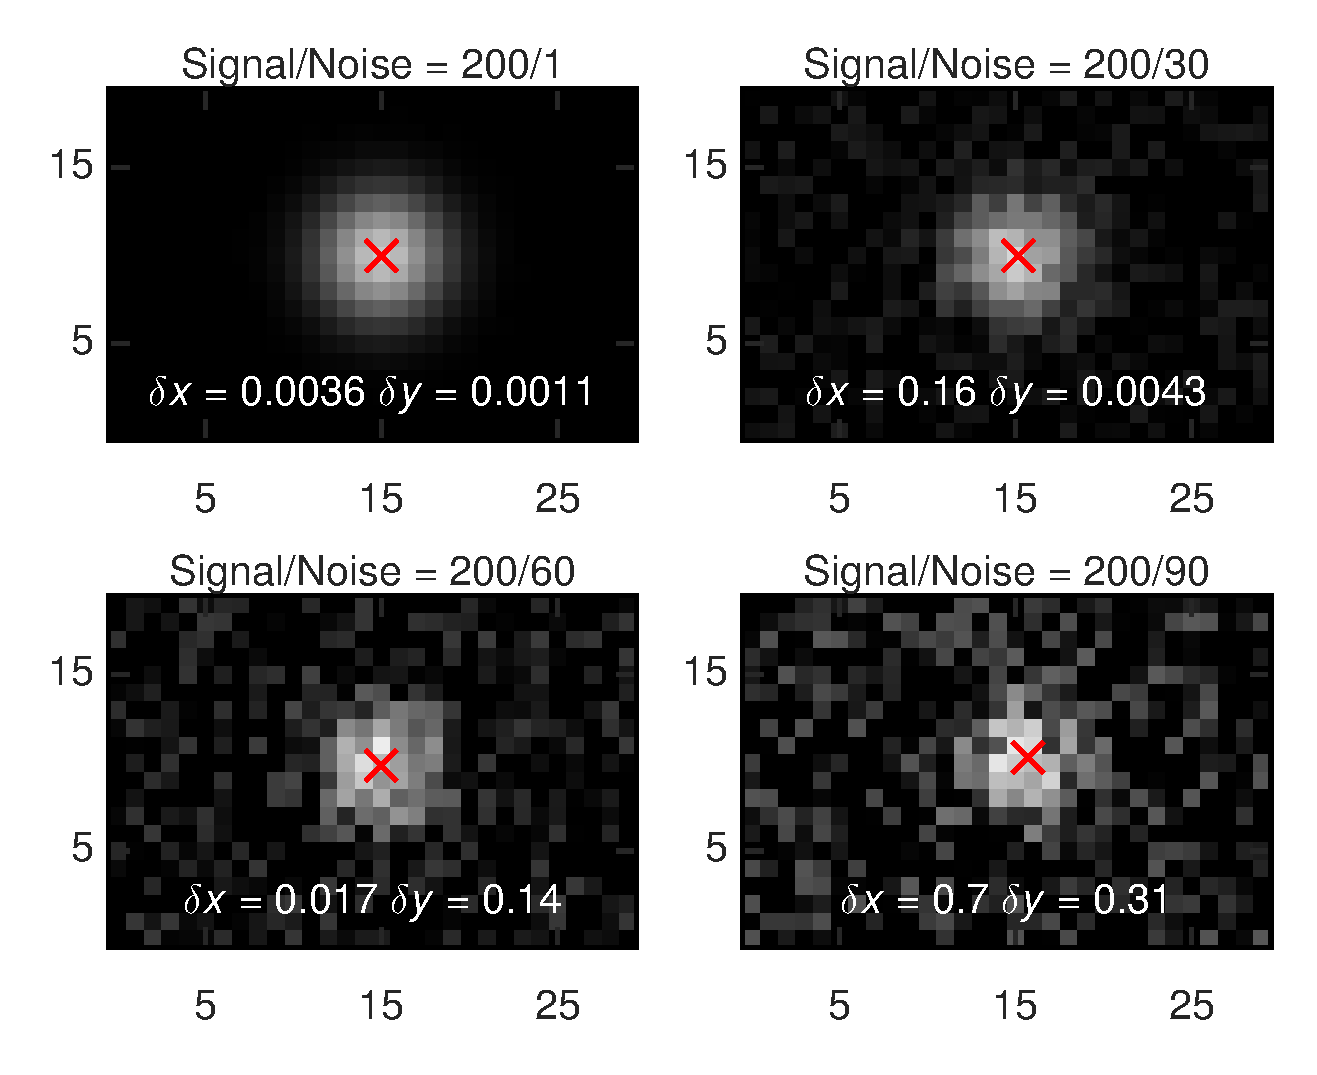
\includegraphics[width=\columnwidth]{trackpy/signal-noise-comparison}
    \caption{\label{fig:static-error}Images depict Gaussian blob with increasing levels of simulated random noise. The red X indicates the measured centroid. Overlaid text gives the error between that measured particle position and the ground truth for each particular example.}
    \end{figure}
    
Simulated images in Figure \ref{fig:static-error} illustrate noisy images and the resultant error in particle location, as realized by trackpy. In simulated images like these, the ground truth is known. In real images, the uncertainty in particle location can be estimated. A relation was worked out in a detailed study of particle tracking errors by Savin and Doyle\cite{Savin2005}. For a hat-like spot, the uncertainty in location is

\begin{equation}
\epsilon = \frac{N}{S}\frac{l_n}{2\pi^{1/2}}\frac{w^2}{a^2}
\end{equation}

\noindent where $N/S$ is noise-to-signal; $l_n$=1 pixel, the length scale of noise correlation; and $w$ and $a$ are, respectively, the apparent size and the size of the neighborhood used to compute the centroid. Trackpy performs this computation for every particle and returns an estimate of $\epsilon$ with the location of every feature it finds. By implementing error analysis as a built-in feature, trackpy encourages researchers to consider this important detail of particle tracking data analysis.

For Brownian motion in a viscous liquid, static error adds a constant offset to the MSD, as derived previously\cite{Martin2002a},

\begin{equation}
\langle \Delta r^2 \rangle_{\text{measured}} = \langle \Delta r^2 \rangle_{\text{true}} + 2\epsilon^2.
\end{equation}

\noindent A perfectly immobilized particle will have $\langle\Delta r^2\rangle_{\text{true}} = 0$ for all lag times, but because of static error, the actual measured MSD will be a non-zero constant, $\langle \Delta r^2 \rangle = 2\epsilon^2$\cite{Martin2002a,Crocker2007}. However, in most particle tracking experiments, the true underlying MSD is not known \emph{a priori}, so it may not be immediately evident how much of the measured MSD is an artifact of noise.

In addition to the random error associated with camera noise and pixelation, particle location is subject to systematic errors, wherein particles can be biased toward certain locations, such as pixel centers. Several experimental details in both hardware and software are implicated in these errors\cite{Crocker2007}. Of course, if the particles typically step much more than a pixel between frames, optimizing subpixel resolution is less important. In this work, they are of greatest importance in characterizing layers exhibiting a solid-like response, when both Brownian vibrations are typically smaller than 1 pixel and convective flow is much slower than 1 pixel per frame.

\subsection{Motion Blur}

Additional error is introduced by the finite  camera exposure time. When a particle moves substantially during the exposure, the recorded image represents the time integral of the particle's location (Figure\ref{fig:motion-blur}). Since particles in random walks tend to revisit previously explored regions, motion during the exposure gives a smoothed trajectory with an MSD that is systematically lower than the true MSD\ref{Crocker2007,Berg1971a}. This effect has been called motion blur and dynamic error \cite{Savin2005}. In addition, particle motion increases static error, because motion blur reduces location precision by roughly two-fold under typical experimental conditions, as compared to stationary particles\cite{Deschout2012}.

   \begin{figure}
    \centering
    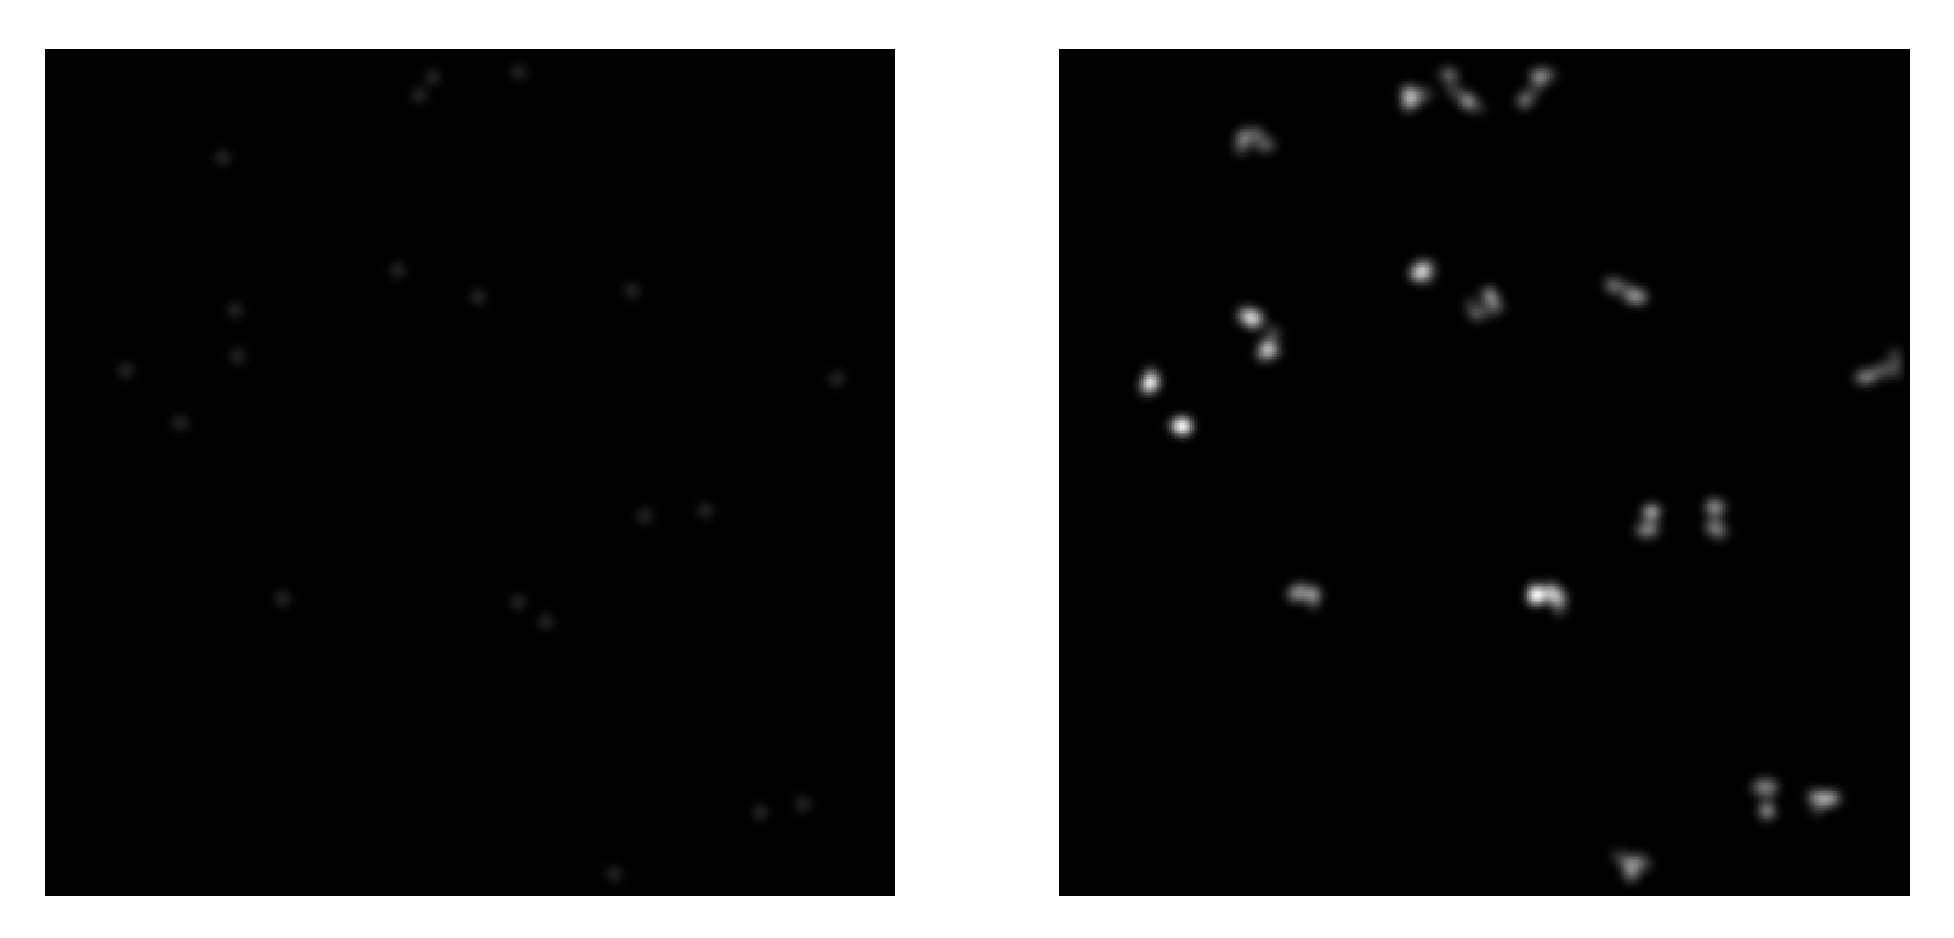
\includegraphics[width=\columnwidth]{trackpy/motion-blur}
    \caption{\label{fig:motion-blur}In these simulated images of diffusing Gaussian blobs, the image on the right was exposed for ten times as long as the image on the left. By collecting more light, it imaged brighter particles, but their precise location is not well defined. The optimal exposure is between these two extremes, as described in the text.}
    \end{figure}

Like static error, dynamic error can alter the measured MSD, and can thus introduce inaccuracies when using the MSD to calculate diffusion coefficients and viscoelastic moduli. Static error alone adds a constant offset to the MSD, which flattens the MSD at short time scales on a log-log plot, and makes diffusive motion appear sub-diffusive\cite{Martin2002a}. Dynamic error, by itself, decreases the MSD at short time scales, which makes diffusive motion appear super-diffusive. Thus, sqtatic and dynamic error distort the MSD in opposite directions, so depending on which type of error is larger, one effect may dominate, or occasionally, the two effects may largely cancel each other \cite{Savin2005}. Both sources of error are more pronounced at short time scales, when the true MSD is smaller.

\subsection{Experimental Best Practices to Minimize Error}
Prior to collecting data, it is critical to consider how to minimize static and dynamic error, as they are difficult to completely correct after the experiment. To boost signal-to-noise ratio and reduce static error, researchers should choose a microscope objective with large numerical aperture and a sensitive camera with low noise. The only way to reduce dynamic error is to use an exposure time that is small compared to the frame interval\cite{Savin2005,Crocker2007}. Unfortunately, shorter exposure time also increases static error. Therefore, for given experimental conditions, one should choose the shortest possible exposure time that still gives high-contrast particles (low signal-to-noise). As a point of reference, \cite{Crocker2007}.for Brownian motion, an exposure time no longer than one quarter the frame interval will cause dynamic error of less than 10\% at the shortest time scale, and smaller dynamic error at longer time scales.

After conducting an experiment, dynamic error is especially difficult to correct, because it distorts the trajectory and MSD systematically in a way that varies with lag time and depends on the underlying type of motion, which is often unknown\cite{Savin2005}. Static error is simpler to quantify and correct after the fact because static error adds a constant offset to MSD regardless of the nature of particle motion. Static error can be estimated by tracking particles fixed to a microscope slide under signal-to-noise conditions similar to those of the experiment, and then subtracted from the ensemble MSD. However, this simple approach may not precisely mimic the background noise in the experiment, nor the effect that motion blur has on static error. An alternative method has recently been proposed for measuring localization precision of moving particles, though this technique requires a custom microscope configuration\cite{Deschout2012}. Tracking particles in water or other fluids of known viscosity and comparing their MSD to theory may also help reveal types and magnitudes of error. 

\section{\label{sec:prediction}Prediction Framework}


The Crocker--Grier particle tracking algorithm, at its simplest level, takes each particle in
a given image and tries to find it in the subsequent image. This
requires knowing where to look for it. The algorithm was developed to track particles undergoing Brownian diffusion,
in which a particle's velocity is uncorrelated from one
frame to the next. Therefore, a particle is statistically most likely to be found at or near is last known location. The particle in a given image closest to a particle in the previous image is likely to be the same particle.

Let us formalize this argument as a \emph{prediction}. Consider a function

\begin{equation}
P(t_1, t_0, \vec x(t_0))
\end{equation}

\noindent that takes the particle at position $\vec x(t_0)$ at time $t_0$ and predicts its most likely 
future position $\vec x(t_1)$ at time $t_1$. The optimal predictor for Brownian motion
is

\begin{equation}
P(t_1, t_0, \vec x(t_0)) = \vec x(t_0)
\end{equation}

\noindent which, of course, is also the simplest to implement.

The better our prediction about where to look in the next frame, the
more likely we will find the one and only particle we seek.
In practice, the algorithm looks for the particle in a circular region of radius
\texttt{search\_range}, centered on $P(t_1, t_0, \vec x(t_0))$. So, a particle is successfully tracked only if its true position at $t_1$ is sufficiently close to the predicted one:

\begin{equation}
\label{eqn:brownian-predictor}
\|P(t_1, t_0, \vec x_i(t_0)) - \vec x_i(t_1)\| \le \tt{search\_range}
\end{equation}

This favors a generous \texttt{search\_range}. However, if
\texttt{search\_range} is too large, then for each particle in the
previous frame there can be many possible matches in the current frame,
and so matching one frame to the next requires the computer to evaluate
an overwhelming set of possibilities, seeking the one that minimizes the total displacements of all particles. Tracking may become extremely
slow, the problem effectively intractable.
So for the Brownian $P$ above, \texttt{search\_range} must be bigger
than the largest particle displacement between frames, but smaller than
the typical spacing between particles\cite{Crocker1996}. If such a value does not exist, the Crocker--Grier algorithm is not effective.

However, if particle motion is not strictly Brownian, its velocity
probably \emph{is} correlated in time. We may be able to improve $P$. This 
is the justification for trackpy's prediction feature.

\subsection{Prescribed predictors}\label{prescribed-predictors}

Consider a toy example: a regular array of particles,
translating with constant velocity $v$. Figure \ref{fig:prediction-const-features}
shows the particles' positions in two consecutive frames.

    \begin{figure}
    \centering
    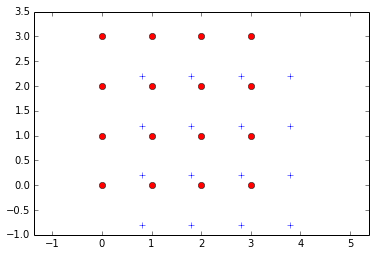
\includegraphics[width=\columnwidth]{prediction/prediction_4_1}
    \caption{\label{fig:prediction-const-features}An ensemble of particles moving under constant velocity. The red circles represent their positions at some time $t$, the blue crosses at some later time $t'$.}
    \end{figure}

\noindent Using the Brownian predictor, Eq. (\ref{eqn:brownian-predictor}), trackpy links the particles as shown in Figure \ref{fig:prediction-const-brownian-link}.

   \begin{figure}
    \centering
    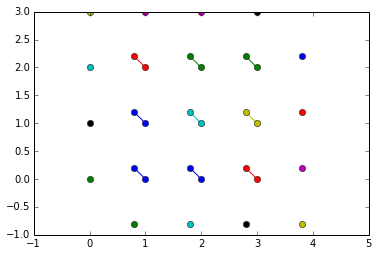
\includegraphics[width=\columnwidth]{prediction/prediction_7_0}
    \caption{\label{fig:prediction-const-brownian-link}An ensemble of particles moving under constant velocity are identified through time using a simple Brownian prediction, Eq. (\ref{eqn:brownian-predictor}). Features that have been identified as belonging to the same trajectory are connected by a line and colored alike. In this case, the identification is not correct.}
    \end{figure}
    
\noindent This is obviously not correct. Let us provide a $P$ which reflects this constant

\begin{equation}
\label{eqn:const-predictor}
P(t_1, t_0, \vec x_i(t_0)) = \vec x_i(t_0) + v(t_1 - t_0)
\end{equation}

\noindent The result is accurate (Figure \ref{fig:prediction-const-const-link}). To be clear, the predictor does not need to specify exactly where the
particle will be; it only must bias the search enough that the correct
identification will be made.

   \begin{figure}
    \centering
    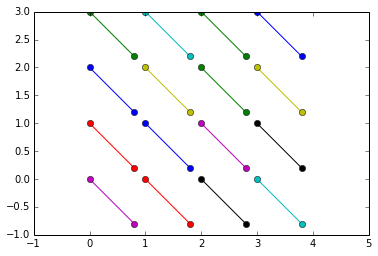
\includegraphics[width=\columnwidth]{prediction/prediction_9_1}
    \caption{\label{fig:prediction-const-const-link}An ensemble of particles moving under constant velocity are identified through time using a constant-velocity predictor, Eq. (\ref{eqn:const-predictor}). As before, Features that have been identified as belonging to the same trajectory are connected by a line and colored alike. }
    \end{figure}

\subsection{Dynamic predictors}\label{dynamic-predictors}

In typical experimental conditions, the particles' velocities are not known ahead of time. It would be much better for the predictor to ``learn'' about
the velocities, and allow different particles to have different
velocities that can change over time. To accomplish this, $P$ will depend on more than $x_0$, $t_0$, and $t_1$; it will also depend on the particles' most recent velocities.

\begin{equation}
\label{eqn:adaptive-predictor}
P(t_1, t_0, \vec x_i(t_0)) = \vec x_i(t_0) + \frac{\vec x_i(t_0) - \vec x_i(t_{-1})}{t_0 - t_{-1}} (t_1 - t_0)
\end{equation}

There are a few caveats.
  If a new particle is in frame $t_i$ but wasn't in $t_{i-1}$, its velocity is unknown, but it is estimated using the velocity of the nearest existing particle. Of course, in the first frame, all
  velocities are unknown because
  there is no previous frame. Fortunately, even though particles may be in motion from the start, an initial guess
  of $v_0 = 0$ often gives acceptable results. In many cases, at
  least some of the particles are moving slowly enough that they can be
  tracked and their velocity can be obtained. Then, because particles with
  unknown velocity borrow the nearest known velocity, this may give the algorithm a foothold to track more particles
  in later frames. If that is not sufficient, a more accurate initial guess can be specified. This guess can be a constant velocity, a velocity profile, or N-dimensional velocity field.

As a demonstration, consider a three-frame sequence that starts
with small displacements and accelerates. With a simple Brownian predictor, tracking fails at the third frame (Figure \ref{fig:prediction-acceleration-brownian-link}). With the adaptive predictor, Eq. (\ref{eqn:adaptive-predictor}), tracking is accurate (Figure \ref{fig:prediction-acceleration-adaptive-link}).


   \begin{figure}
    \centering
    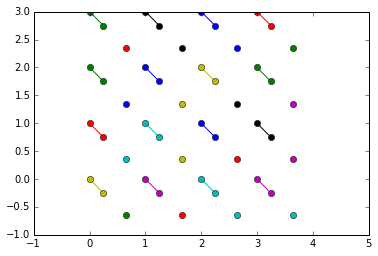
\includegraphics[width=\columnwidth]{prediction/prediction_14_1}
    \caption{\label{fig:prediction-acceleration-brownian-link}An ensemble of accelerating particles are identified through time using a simple Brownian prediction, Eq. (\ref{eqn:brownian-predictor}). As before, Features that have been identified as belonging to the same trajectory are connected by a line and colored alike. The identification is incorrect.}
    \end{figure}
   

   \begin{figure}
    \centering
    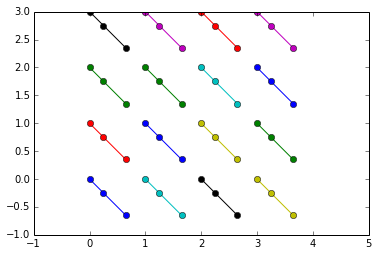
\includegraphics[width=\columnwidth]{prediction/prediction_16_1}
    \caption{\label{fig:prediction-acceleration-adaptive-link}An ensemble of accelerating particles are identified through time using a simple Brownian prediction, Eq. (\ref{eqn:adaptive-predictor}). As before, Features that have been identified as belonging to the same trajectory are connected by a line and colored alike. }
    \end{figure}


    \subsubsection{Channel flow prediction}\label{channel-flow-prediction}

There are two special cases implemented by trackpy. The first is channel flow, in which velocities are relatively uniform in one
direction. For example, if the channel is in the $x$ (i.e. $\hat i$)
direction, particle velocities are very well approximated as

\begin{equation}
\vec v = \hat i v_x(y)
\end{equation}

\noindent where the velocity profile $v_x(y)$ is a smoothly-varying function
defined across the channel. The required inputs are the direction of flow and size of the bins used to
define the channel profile. The initial velocities can be specified or arrived at adaptively.

Figure \ref{fig:prediction-channel-brownian-link} shows an example. The simple Brownian prediction fails for the top row of particles at the center of the channel. With a Channel Flow prediction, the tracking is accurate (Figure \ref{fig:prediction-channel-channel-link}).

   \begin{figure}
    \centering
    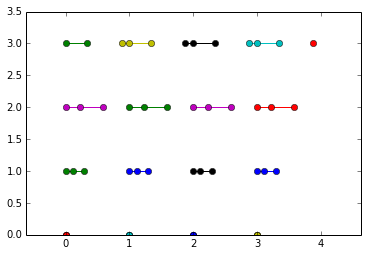
\includegraphics[width=\columnwidth]{prediction/prediction_20_1}
    \caption{\label{fig:prediction-channel-brownian-link}An ensemble of particle moving in simulated channel flow are identified through time using a simple Brownian prediction, Eq. (\ref{eqn:brownian-predictor}). As before, Features that have been identified as belonging to the same trajectory are connected by a line and colored alike. The identification is incorrect.}
    \end{figure}

   \begin{figure}
    \centering
    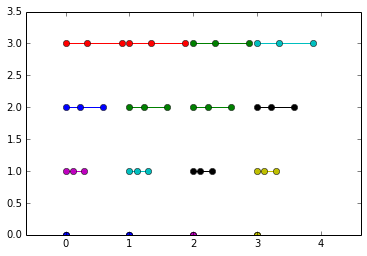
\includegraphics[width=\columnwidth]{prediction/prediction_22_1}
    \caption{\label{fig:prediction-channel-channel-link}An ensemble of particle moving in simulated channel flow are identified through time using a Channel Flow predictor. As before, Features that have been identified as belonging to the same trajectory are connected by a line and colored alike. }
    \end{figure}

    \subsubsection{Drift prediction}\label{drift-prediction}
    
The second special case implemented by trackpy is drift prediction. In interfacial microrheology measurements, it is common to observe convective flows driven by air currents or heat from the illuminating lamp. During data analysis, this motion can often be subtracted by adopting a reference frame set by the average velocity of the ensemble of particles. Likewise, tracking accuracy and performance is improved by forming a prediction based on the average velocity of the ensemble.

\section{\label{sec:testing}Testing \& Reproducibility}

Trackpy is packaged with more than 180 automated tests: snippets of code that exercise a specific capability of trackpy by running toy examples and comparing the output to known correct results. For example, to test feature location, an automated test draws a simple image with several dots and checks that trackpy can locate the dots with a given precision.

Testing benefits a research code in more than one way. Most obviously, tests verify correctness and check special cases. Just as important, tests protect reproducibility. By codifying key results as tests, authors can be sure that these results cannot be broken inadvertently in the future. This empowers users who do not have familiarity with the whole codebase to make contributions and changes with confidence that they will not have unintended consequences. When revisions are submitted to trackpy, a web service automatically executes all the tests, and it alerts the user if any tests fail under the proposed change. Finally, the test suite complements the documentation. Technical users and potential contributors can browse it as a comprehensive demonstration of the ways in which the authors imagined the code would be used.

Trackpy has an unusual level of testing for a code from an academic lab. But the time invested has been worthwhile: it ensures that any research that depends on the code is grounded in a rigorous, scientific approach to software development. This guarantee earns the confidence of other researchers who decide to use, cite, or contribute to the codebase. It thereby increases the code's longevity and the impact of the development effort.

As trackpy is improved and changed, old research code may cease to reproduce exactly the same results. Testing help ensure that any such ``breaking changes'' are made deliberately and can be documented. To avoid breaking old code altogether, researchers can make note of which specific version of trackpy was used for a given project and roll back to that version when revisiting the research. Several new projects such as Docker, Dexy, and hashdist address this need: they recreate complete computing environments, making it possible reproduce research using the specific original versions of all the relevant software. These tools are especially powerful in simulation research, where the entire research project can reproduced on a computer. But, they are also useful in experimental science, covering every step after data collection up to the production of the published figure.

\section{Conclusion}
\subsection{``A Modern Approach''}
Trackpy is distinguished among niche academic codes by its careful adherence to the best practices of the open source software community\cite{Wilson2014a}. The most important are code review and open discussion before each revision, automated testing, complete API documentation. Also, code comprehensibility and modularity are key design considerations. Code that merely works is not necessarily easy to test, maintain, extend, or reuse.

Code for academic use is typically developed for a single research project, often by a single researcher, at least at first. Trackpy has benefitted from its co-development by three different researchers working in separate groups at separate institutions on projects with vastly different priorities. The core functionality of trackpy was useful to all, and the healthy tension in the project drove the development of extensible, reusable code. In addition to the core developers, collaborators and other researchers used trackpy actively during its development. Their use of the cutting-edge code demanded stability and thorough documentation. As the project matured, a wider community of users discovered it and found it useful.

\subsection{Measuring Success}
The scientific software community has not settled on a single metric for the success of academic software. In the three years since the first lines of code were written, trackpy has supported published research from several academic research groups; trackpy has been downloaded thousands of times through the Python Package Index, though it is impossible to know if the recipients were genuine users; trackpy has been adopted by users from about ten top academic research institutions known to the authors. Most importantly, trackpy has benefitted from code contributions offered by those users, comprising both software experts and relative novices. Particle tracking is a general problem in a number of fields, and thanks to the pioneering efforts of John Crocker, David Grier, and Eric Weeks, it has a strong tradition of open source code supporting first-rate research.

\subsection{Future Directions}

Trackpy can increase its impact and extend its applicability by incorporating algorithms and strategies from outside the colloids literature and the software lineage of Crocker and Grier. Researchers in the biological and biophysics communities also use these tools, but they have developed additional methods to solve more complicated image analysis problems. For example, in biological contexts, features must be located amidst a complex, busy environment where they are more difficult to distinguish and the methods discussed above can be insufficient to extract them. Tracking and the notion of a trajectory can be subtler, as features might split or merge with each other.

Separately, the scientific Python community continues to grow and develop ever more powerful tools for exploring, processing, and presenting data. Trackpy will build on this ongoing progress, providing tools specific to the needs of particle tracking.